\chapter{Lösungsvorschläge}
In diesem Kapitel werden die
\section{Implementierung eines Ruby on Rails Content Repository}

Die hier betrachteten WCMS haben bei der Speicherung ihrer Daten teilweise sehr einfache Modelle inenrhalb einer
Einen Möglichen Lösungsansatz bietet dabei die Umsetzung eines Content Repository. Im folgenden sollen die Konzepte dieser Lösung vorgestellt und die Vorteile für die bestehenden Ruby on Rails Content Management Systeme formuliert werden.


\subsection{Idee und Konzept}

Heutige Anwendungen (u.a. auch Web Content Management Systeme) benötigen neben der klassischen Speicherung von Daten zahlreiche zusätzliche Daten Management-Funktionalitäten. Ein Content Repository erweitert bestehende Datenbanken u.a um folgende zusätzlichen Funktionalitäten:

\begin{itemize}
\item
Speicherung strukturierter und unstrukturierter Daten (z.B. Binär- und Textformate oder Metadaten)
\item
Zugangskontrolle
\item
Sperrung (Locking)
\item
Transaktionen
\item
Versionierung
\item
Überwachung der Daten
\item
Volltextsuche
\end{itemize}

Im Bereich der Java Enterprise Content Management Systeme werden Content Repositories bereits erfolgreich eingesetzt. Namhafte Beispiele sind dabei das kommerzielle ECMS CQ5 und CRX\footnote{Nach der Übernahme von Day Inc. durch Adobe im Sommer 2010 wird das angebotene Content Management System CRX als Adobe Projekt weitervertrieben.} von Adobe und das u.a. als Open Source verfügbare Alfresco ECMS\footnote{Informationen zu Alfresco und dem Content Repository: \href{http://www.alfresco.com/products/platform/}{http://www.alfresco.com/products/platform/}}.
Innerhalb der PHP-Entwicklergemeinde wird ebenfalls gerade an der Umsetzung eines auf PHP basierten Content Repositories gearbeitet. Initiatoren sind dabei vor allem die Typo3 Assocation mit ihrer Umsetzung innerhalb des neuen Web Content Management Systems Typo3 5.0.


\subsection{Das Java Content Repository}

Unter der Leitung von David Nuescheler der Firma Day Software wurde 2005 die erste Version einer Implementierung und einer API Spezifikation eines Java Content Repository veröffentlicht\footnote{Die Entwicklung ging im Java Specification Request (JCR) 170 als offizieller Standard in die Programmiersprache Java ein. Momentan wird an der Veröffentlichung der Version 2.0 des Standards gearbeitet(JSR-283).}. Die umgesetzte Referenzimplementierung wurde später unter der Leitung der Apache Foundation als Open Source Projekt Jack Rabbit\footnote{Homepage: \href{http://jackrabbit.apache.org/}{http://jackrabbit.apache.org/}} der Öffentlichkeit zur Verfügung gestellt.


\subsection{Umsetzungsvarianten innerhalb von Ruby on Rails}

Durch die Verfügbarkeit eines Ruby-Interpreter in Java (jruby) ergeben sich für die Umsetzung in Ruby on Rails folgende 2 Möglichkeiten:

\begin{itemize}
\item
Verwendung der Open Source Java Implementierung Jack Rabbit und Spezifkation einer API zur Nutzung dieser innerhalb von Rails.
\item
Erstellung einer eigenständigen, komplett auf Ruby basierenden Referenzimplementierung und API nach dem Vorbild des Java Content Repository
\end{itemize}



\subsection{Vorteile für die gewählten Ruby on Rails WCMS}

Die Umsetzung eines Content Repository in Ruby kann für Web Content Management Systeme folgende Vorzüge bringen:

\begin{itemize}
\item Vereinfachung des Zugriffs auf Inhalte innerhalb verschiedener Systeme
\item Durch die im JCR Standard festgelegten Import- und Exportfunktionen kann ein Austausch der Inhalte zwischen einzelnen Web Content Management Systemen ermöglicht werden. Der momentane Mangel an standardisierten Exportfunktionen in den Systemen kann so ebenfalls beseitigt werden.
\item

\end{itemize}



\section{Übertragung des Typo3 5.0 Phoenix User-Interfaces in Rails 3.1}
Content Management Systeme erfordern bei steigender Funktionalität ein entsprechend komplexeres Nutzer-Interface. Die sinnvolle Realisierung entsprechender Oberflächen ist mit der u.a. in Refinery CMS gewählten Generierung von HTML-Views und einzelnen JavaScript-Dateien nur noch schwer möglich. Zur Umsetzung solcher Projekte empfiehlt sich daher der Einsatz alternativer Technologien.
Die neue Version 5.0 des PHP basierten Web Content Management Systems Typo3 greift bei der Generierung der gesamten Backend-Oberfläche auf das Java Script Frameworks Ext JS 4\footnote{Informationen und Download: \href{http://www.sencha.com/}{http://www.sencha.com/}} zurück. Es ermöglicht durch Kombinierung vorgefertigter Elemente eine schnelle Erstellung komplexer Oberflächen\footnote{Beispielanwendungen: \href{http://dev.sencha.com/deploy/ext-4.0.0/examples/}{http://dev.sencha.com/deploy/ext-4.0.0/examples/}}.
Die Veröffentlichung des Typo3-Projektes unter der GPLv3-Lizenz macht eine Weiternutzung der in der Version 5.0 geplanten Oberfläche generell möglich. Im folgenden sollen daher die notwendigen Schritte zur Integrierung des Typo3 5.0 User-Interfaces in eine Rails 3.1 Anwendung beschrieben werden.

\subsection{Typo3 5.0}
Die Entwicklung von Typo3 5.0 befindet sich noch in einer frühen Phase. Interessenten können jedoch bereits Entwicklerversionen in Form sogenannter Sprint Releases herunterladen und testen. Neben einem Download-Paket\footnote{Komponenten-Download: \href{http://flow3.typo3.org/typo3-phoenix/}{http://flow3.typo3.org/typo3-phoenix/}} auf der Projektseite von Typo3 wird zusätzlich eine aktuelle Version von Typo3 als Live-Demo\footnote{Demoseite: \href{http://phoenix.demo.typo3.org/}{http://phoenix.demo.typo3.org/}} angeboten. Die Zugangsdaten zum Backend können im Frontend der Seite mit Hilfe eines Formulars erzeugt werden.


\begin{figure}[!h]
\begin{center}
\label{fig.typo3frontend}
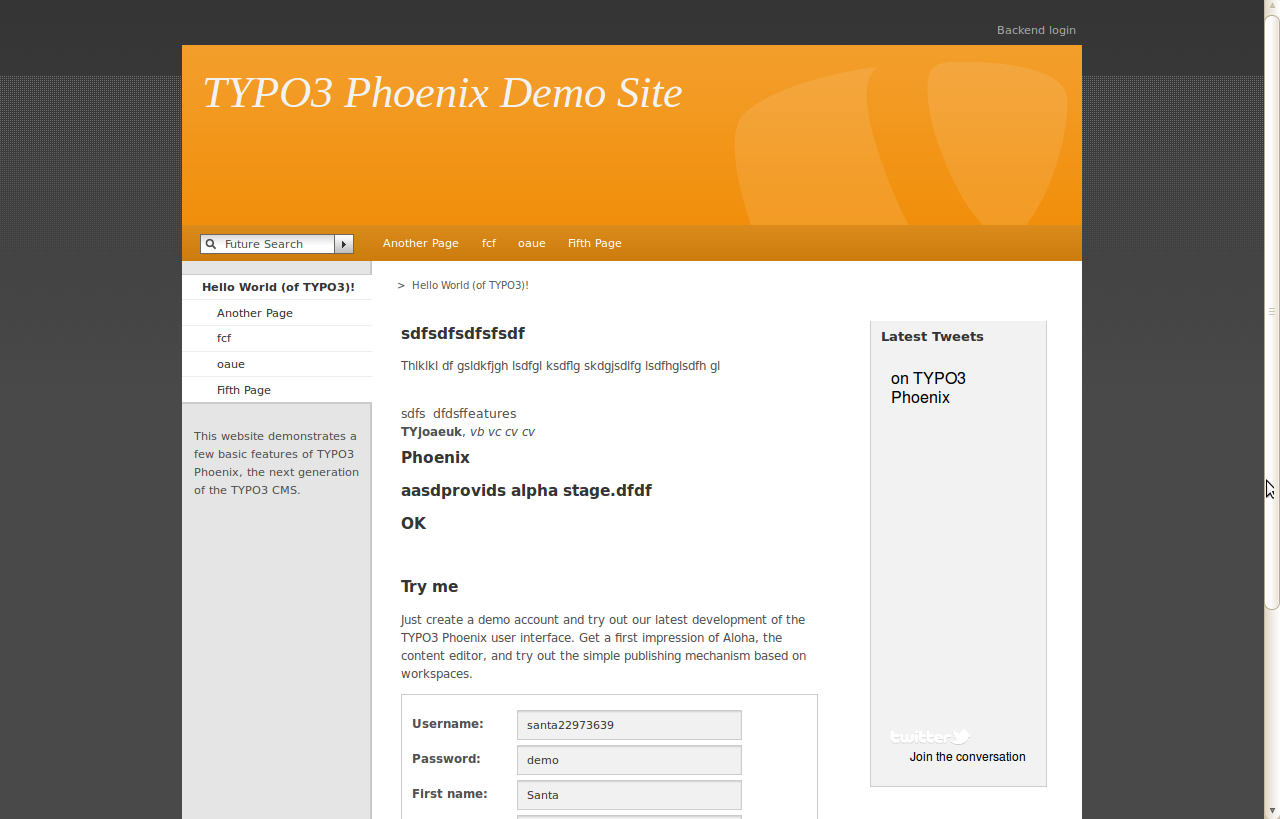
\includegraphics[scale=0.239]{images/typo3/frontend.png}
\caption{Frontend-Ansicht der Typo3 5.0 Sprint Release 6 Demoversion}
\end{center}
\end{figure}


\begin{figure}[!h]
\begin{center}
\label{fig.typo3backend}
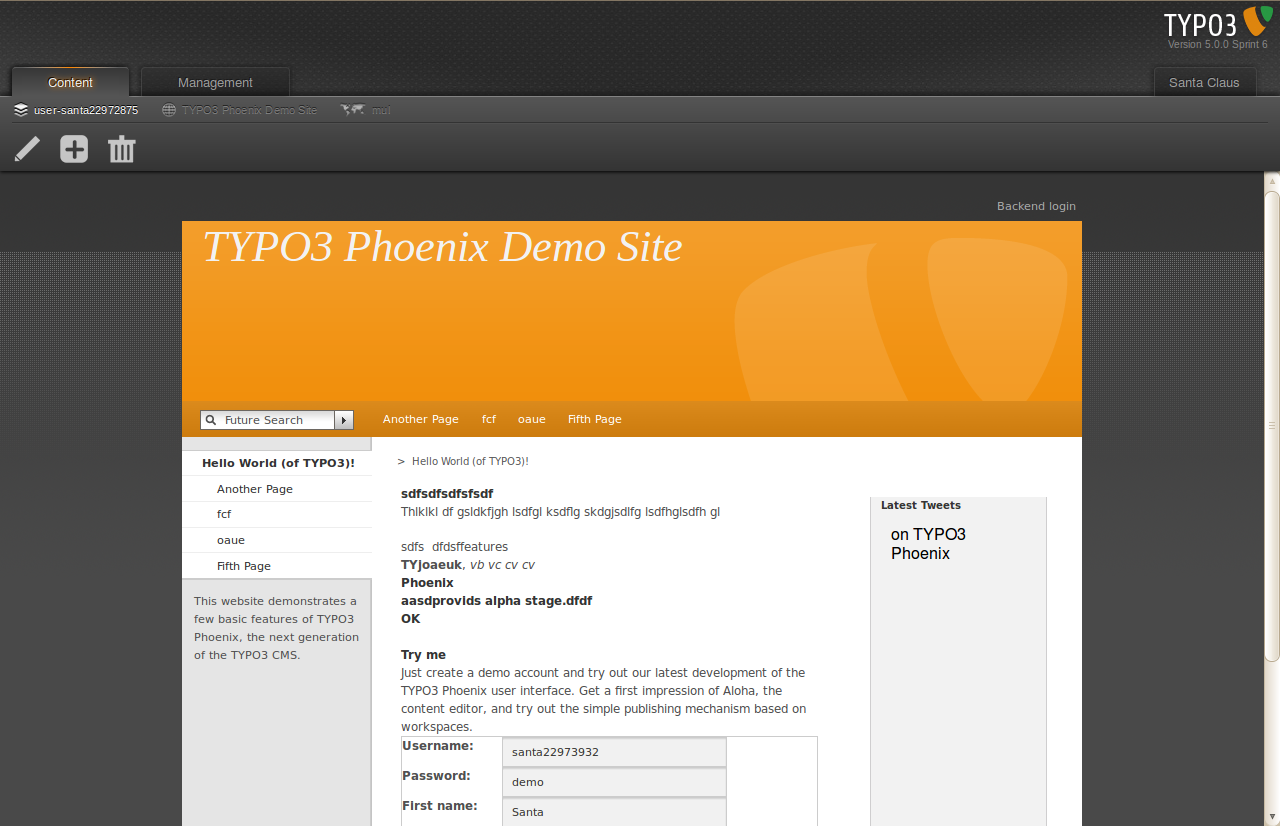
\includegraphics[scale=0.239]{images/typo3/backend.png}
\caption{Backend-Ansicht der Typo3 5.0 Sprint Release 6 Demoversion}
\end{center}
\end{figure}
\newpage
Das in der Demoversion umgesetzte Nutzer-Interface repräsentiert nur einen Teil der für Typo3 5.0 geplanten Oberfläche und Komponenten\footnote{Bilder und ausführliche Erläuterungen zur neuen Typo3 5.0 Oberfläche sind unter folgender Adresse zu finden: \href{http://typo3.org/teams/usability/t35ui/}{http://typo3.org/teams/usability/t35ui/}}. U.a. sind folgende Bestandteile bereits umgesetzt wurden:
\begin{itemize}
\item
Login-Seite zur Anmeldung im Backend von Typo3 5.0
\item
Content-Modul im Backend mit integrierter Vorschau der aktuell ausgewählten Seite und beschränkten Möglichkeiten der
Inhaltsbearbeitung mit Hilfe des für Typo3 5.0 geplanten Aloha-Editors
\item
Management-Modul zur Verwaltung der im System angelegten Seiten in Form einer Baumstruktur
\item
Dashboard des angemeldeten Nutzers mit Auflistung der editierten Inhalte
\end{itemize}


\subsection{Ext Js mit Ext Direct}
Mit Hilfe des Ext Js Frameworks können einzelne Komponenten zu einer großen Oberfläche zusammengebaut werden. Die Befüllung der Oberfläche mit Daten vom Server erfolgt dabei asynchron in Form sogenannter Ajax-Anfragen (Ajax Requests).

